%%% There's not a lot of extra documentation in this file, other than
%%% the text itself.  On the other hand, you may be looking for
%%% a few examples of how to insert figures, so go ahead and peruse.

\chapter{Working with Graphics}

In this chapter, we'll be dealing with the inclusion and placement of
figures and other graphics in your thesis.  Usually a figure will be a
graphic of some type (e.g., a photograph, line drawing, chart) that
resides in a separate file external to your document.  You will need
to decide on a format for these figures.  If you are generating your
own graphics using other programs, you may have the option to choose
the output format.  Otherwise, you may need to use other software to
convert the graphic into a compatible format for inclusion in your
\LaTeX{} document.

\section{Raster and Vector Graphics}
Graphics for print media are generally in one of two classes: raster
images or vector drawings.  A \acro{JPEG} photograph is an example of
a raster format, where a matrix of pixels has a defined value.  Raster
images may be scaled up or down in size, but within limits. Scale such
an image too large and it will become ``pixelated'' or blocky.
Reduce the image too much, and finer details will be blurred or lost.
If you use raster images in your thesis, they should be generated with
a sufficiently high resolution that scaling artifacts will be
minimized.  For print media, a resolution of 300 to 600\,dpi (dots per
inch) might be typical.  For viewing on screen, a minimum resolution
of 100\,dpi may be adequate.  \acro{PNG}, \acro{JPEG} and \acro{GIF}
images are common examples of a raster type.  PhotoShop, The Gimp, and
other paint-type or photo-manipulation programs typically generate
raster images.  Scanning documents or other graphics will also
generate a raster image of some kind, usually in one of \acro{JPEG},
\acro{TIFF}, or \acro{PDF} formats.

In contrast, vector images will scale better.  Vector images are
usually line-drawings, text, and many kinds of graphs.  Vector images
can be scaled better because the pixel values are not defined until
after the scaling occurs, so the image can be rendered at the full
resolution of the output device, whether it be for print or screen.
Also, vector images are often encoded in a much smaller space than a
comparably-sized raster image.  Adobe Illustrator, CorelDRAW,
Inkscape, and Flash are examples of programs that generate vector
images.  \acro{WMF} and \acro{SVG} are also common vector formats,
though these types of files may not be included in your documents
directly: they must be first converted to another file format.

In generating figures for your document, if you have a choice, choose
a vector format, since it will provide the best scaling flexibility.
(See figure~\ref{ex-complete} for an example of a vector drawing.)
However, if you must include a photograph or scanned document of some
type, then be sure that the raster image has a sufficiently high
resolution for the intended publishing medium. (Figure~\ref{franklin}
is an example of a \acro{JPEG} raster image.)

\section{The \pkg{graphicx} Package}
The \LaTeX{} package \pkg{graphicx} allows you to insert external
PostScript or other files into your document.  There are other
figure-inclusion packages that you can use, but \pkg{graphicx} is
probably the most commonly-used, providing several useful features for
the task.

Using the MiK\TeX or Mac\TeX packages, you are probably using the
\lit{pdflatex} program to create a \acro{PDF} document directly from
the file sources.  If you look back at this document's ``driver'' file
\lit{thesis.tex}, you'll find a line that says
\verb|\usepackage[pdftex]{graphicx}|.  The option \lit{pdftex}
indicates that the \pkg{graphicx} package should employ the
\lit{pdftex} version of the driver to insert figures in a manner
compatible with the pdf\LaTeX{} processor.  Using this driver, all of
your external figures will need to be in \acro{PDF}, \acro{PNG},
\acro{JPEG}, or \acro{GIF} format.  Other types of graphics files will
need to be converted to one of these formats before they may be
included in your document.

An alternative driver to \lit{pdftex} is the option \lit{dvips}, which
will require all your figures to be in Encapsulated PostScript
(\acro{EPS}) format.  Other formats will need to be first converted to
PostScript.  (Both PostScript and \acro{PDF} formats may contain
either raster or vector images, or even both at once.)  This is the
driver you should use if you are using the program \lit{latex} instead
of \lit{pdflatex} to process your document.  The \acro{DVI} output
from the \lit{latex} program is later processed by the \lit{dvips}
program to convert the output to PostScript, which may then be
converted to \acro{PDF}.  If you have lots of figures in PostScript
format already, or if you will be using one of many \LaTeX\ packages
that creates PostScript figures, you may need to use this driver (and
you probably know what you're doing already).

For the purposes of this sample document, the figures are provided in
both \acro{EPS} and \acro{PDF} forms, so you may choose to use either
the $\mbox{\lit{latex}}\rightarrow\mbox{\lit{dvips}}$ command chain,
or \lit{pdflatex} to process this document. In fact, there's some
fancy code in the \lit{thesis.tex} file that chooses the right driver
depending on whether you're running \lit{pdflatex} or \lit{latex} on
these source texts.

\section{PostScript, Encapsulated PostScript, and PDF}
PostScript is a programming language for putting marks on a page.  As
such, PostScript files can usually be edited using plain text editors,
should that ever be necessary.  A file containing Encapsulated
PostScript conforms to additional standards, allowing the graphic to
be manipulated or included in other PostScript programs more readily.

As far as \LaTeX{} is concerned, the most important feature of an
Encapsulated PostScript file is the \lit{\%\%BoundingBox}, which is
defined as the smallest rectangle that completely encloses the figure.
Two sets of $x$- and $y$-coordinates describe the bounding box; the
first $(x,y)$ pair gives the lower left-hand coordinates of box
relative to the bottom left-hand corner of the page, and the second
pair of coordinates identify the upper right-hand corner of the
bounding box.  You normally don't have to worry about this information
at all, but if a PostScript figure does not contain
\lit{\%\%BoundingBox} information, or if the \lit{\%\%BoundingBox} is
incorrect, the \pkg{graphicx} package allows you to specify the
bounding box coordinates yourself when you insert the figure into your
document.

A \acro{PDF} figure will have its dimensions embedded within it
already, so you will not need to make any special preparations to
include it in your document. \acro{PDF} has a lot in common with
PostScript, and the two formats may be converted from one to the
other, usually without any loss in quality.  Depending on your
distribution of \LaTeX, you may have a program already installed which
converts \acro{EPS} files to \acro{PDF}.  One of the simplest
converters is the program \lit{epstopdf}, which can be executed as
follows:
\begin{verbatim}
epstopdf myfig.eps
\end{verbatim}
A Windows version of this program might pop up a user interface for
fine-tuning the figure conversion, while the Unix/Linux version of the
program will simply do the conversion, creating \lit{myfig.pdf}
without any intervention required.

\section{Inserting Figures}
The basic mechanics of including a PostScript graphic (\lit{dvips}
driver) or \acro{PDF} graphic (\lit{pdftex} driver) are relatively
simple:
\begin{verbatim}
\includegraphics{figurefile}
\end{verbatim}
This command will insert the graphic contained in the file
\lit{figurefile} at that particular location in the text.  The file
name may have optional extensions, depending on the driver.  For
example, the \lit{dvips} driver will recognize the \lit{.ps} or
\lit{.eps} file extensions, while the \lit{pdftex} driver will
recognize extensions \lit{.pdf} and \lit{.jpg}.  \LaTeX{} will leave
space for the graphic according to the bounding box information that
the file contains.

For inclusion in your thesis or dissertation, a graphic will normally
be labeled and given a caption.  To do this, you will wrap the
\verb|\includegraphics| command in a \lit{figure} environment.
Figures will usually ``float'' from the location where they were
defined.  By default, \LaTeX{} will try to place figures at the bottom
of the current page (if there's sufficient room), then at the top of
the next available page.  Failing that, \LaTeX{} will place figures
onto their own page.  The \verb|\caption| command will number the
figure automatically.  If you need to refer to the figure in your
text, include a \verb|\label| command following the \verb|\caption|,
and then use the \verb|\ref| and \verb|\pageref| commands to
retrieve the figure number and figure's page number, as required.

As a complete example, refer to Figure~\ref{ex-complete}.  I used the
following commands to include the figure graphic:
\begin{verbatim}
\begin{figure}
\begin{center}

\includegraphics[scale=0.6]{figs/fleur}
\end{center}
\caption{This is a simple figure, ...}
\label{ex-complete}
\end{figure}
\end{verbatim}
In this case, the graphic file is located in the folder \lit{figs},
and the complete file name is either \lit{fleur.eps} or
\lit{fleur.pdf}. If I'm using the \lit{dvips} driver, the \lit{.eps}
extension is added automatically; likewise, the \lit{.pdf} extension
would be added if I am using the \lit{pdftex} driver.  To
center the graphic horizontally, I enclosed the
\verb|\includegraphics| command in a \lit{center} environment. The
\verb|\caption| command handles text like this: a short, one-line
caption will be horizontally centered, and a longer caption will be
broken into multiple lines as required, with narrower margins.

At the beginning of the previous paragraph, I typed
\verb|Figure~\ref{ex-complete}| to retrieve the figure number.  If I
use this mechanism for all of the equations, tables, and figures in my
manuscript, I never have to worry about renumbering anything should I
choose to move blocks of text or figures around.  I can also state that
Figure~\ref{ex-complete} will be found on page~\pageref{ex-complete}
by typing
\begin{verbatim}
Figure~\ref{ex-complete} will be found on page~\pageref{ex-complete}
\end{verbatim}

\begin{figure}
\begin{center}

\includegraphics[scale=0.6]{figs/fleur}
\end{center}
\caption{This is a simple figure, but a complete example. This figure
is a vector drawing, so it may be scaled up or down without loss of
precision.}
\label{ex-complete}
\end{figure}


this is jian wang
The \verb|\includegraphics| command has several optional arguments
which will allow you to adjust figure position, bounding box,
rotation, scaling, and other elements, without having to edit the
figure itself.  Figure~\ref{franklin} displays an image in its raw
state, and then a close-up, rotated image of a segment of the same
PostScript graphic.  A complete description of the all the options
available is best left for the \pkg{graphicx} package manual page, but
the transformed image was accomplished with the following
\verb|\includegraphics| line:
\begin{verbatim}
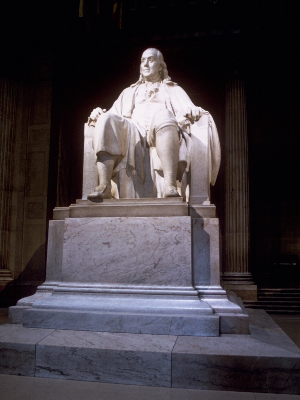
\includegraphics[viewport=.9in 2.1in 1.15in 2.35in,clip,
    scale=10.67,angle=90]{figs/ben}
\end{verbatim}

\begin{figure}
\begin{center}
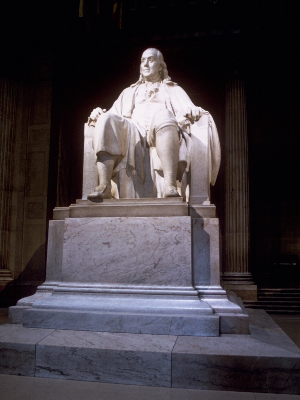
\includegraphics{figs/ben}
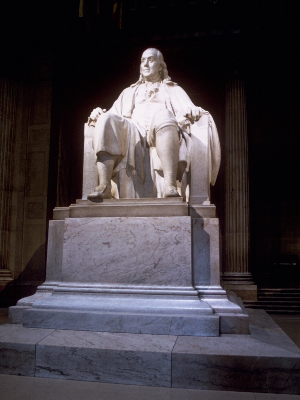
\includegraphics[viewport=.9in 2.1in 1.15in 2.35in,clip,
    scale=10.67,angle=90]{figs/ben}
\end{center}
\caption{Benjamin Franklin, in raw form (left), and close-up and
  rotated (right).  (Notice that the close-up figure displays
  ``pixelation'' effects of a raster image scaled too large.)}
\label{franklin}
\end{figure}

\section{Inserting Forms or Full-Page Figures}
If you need to include a copy of an approval form or certification in
your document, you can take advantage of a few additional options of
the \verb|\includegraphics| command to allow the figure to occupy most
of the page.  If you already have an electronic version of a full-page
form, you can eliminate some of the white space border of the
page before insertion to reduce the amount of scaling required.
As an example, the file \lit{rights} in the \lit{figs} folder is a
full page of text with 1-inch borders on all sides.
I can tell \verb|\includegraphics| to trim this space and fill
the rest of the page with a command like this:
\begin{verbatim}
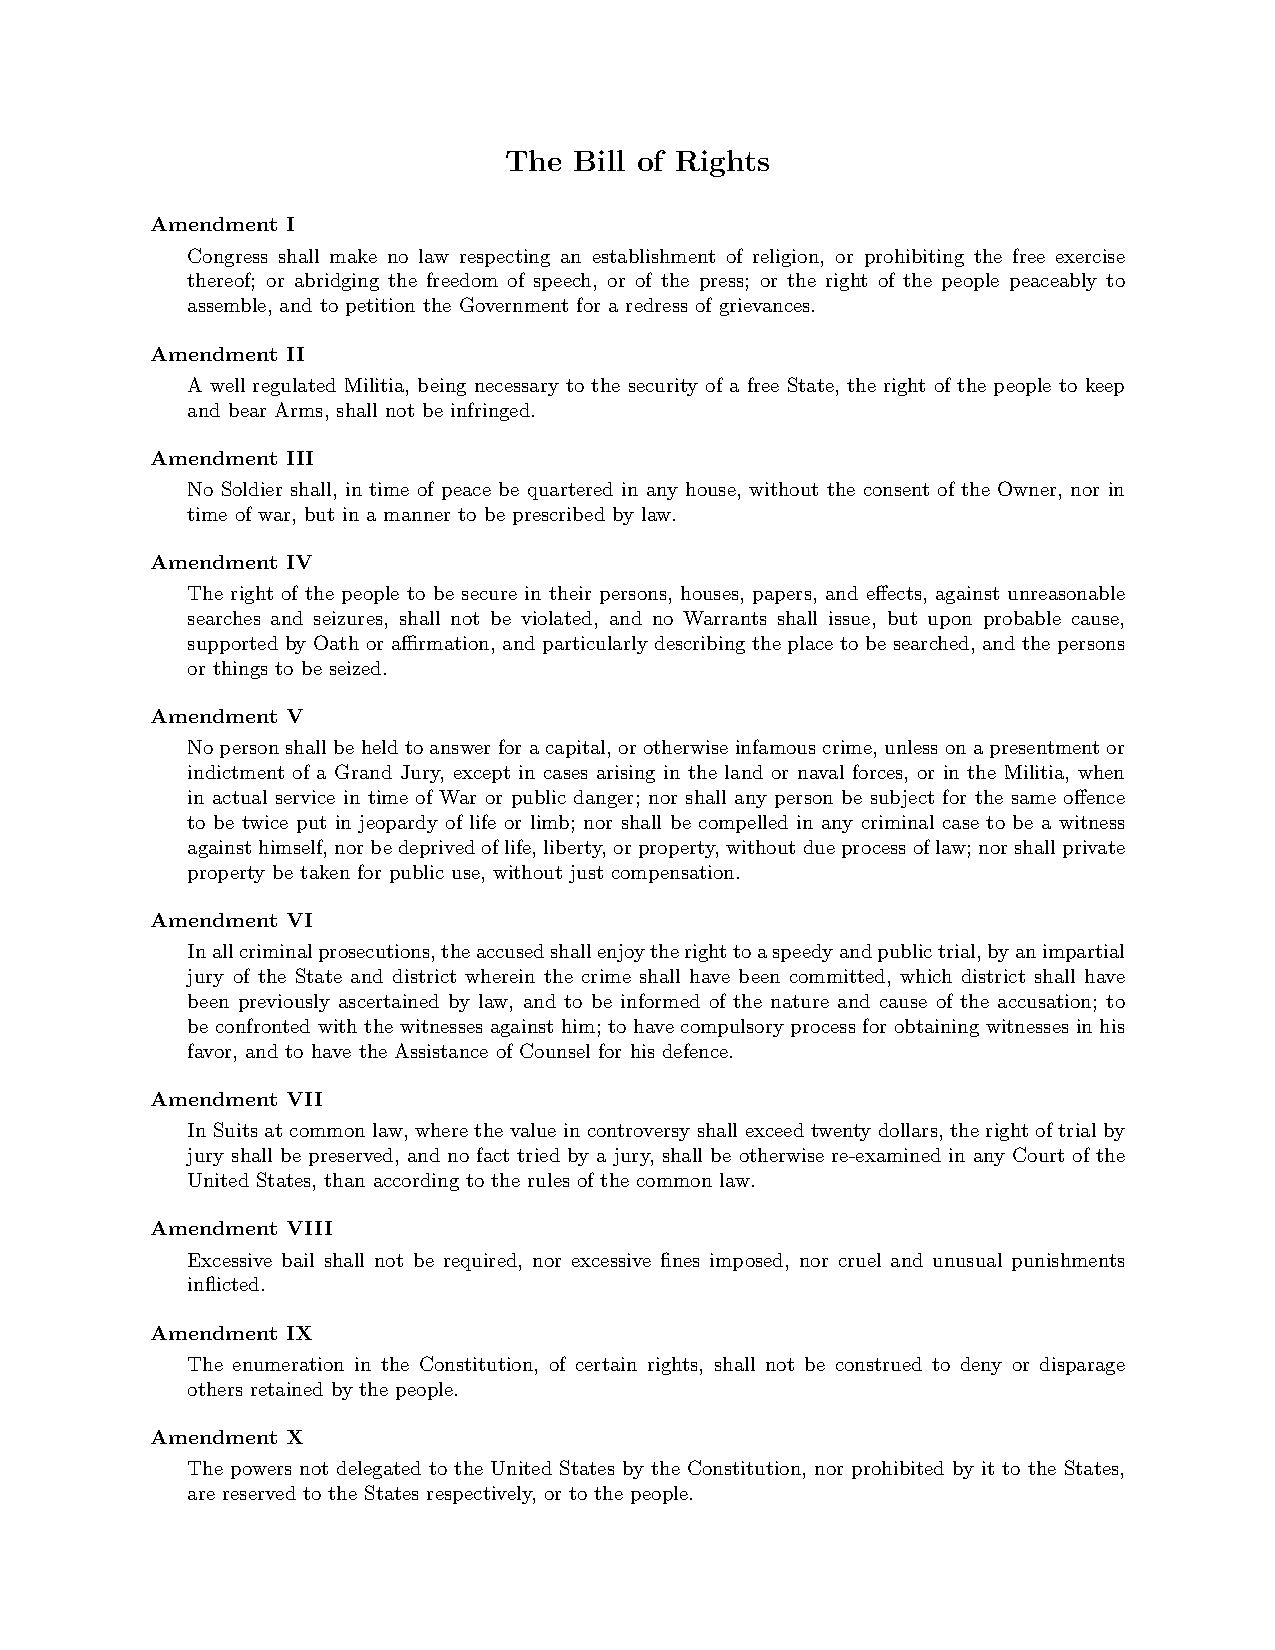
\includegraphics[trim=1in 1in 1in 1in, clip,
    height=\textheight]{figs/rights}}
\end{verbatim}

The \verb|trim| and \verb|clip| options remove the whitespace border.
The \verb|height=\textheight| command stretches or compresses the
figure to the full text column height, allowing room for the page
number. On the other hand, if the full-page image needs a caption,
you'll need to reduce the scale a bit more to fit it in.  In addition,
I could draw an outline around the figure with an \verb|\fbox| command
to give it a page-within-a-page appearance.  In this case, I might
want to leave a small amount of whitespace around the text of the
inserted page.  Making these modifications and leaving a bit of room
for the caption gives us the commands below.  You can see the results
on page~\pageref{fig:rights}.
\begin{verbatim}
\begin{figure}
\fbox{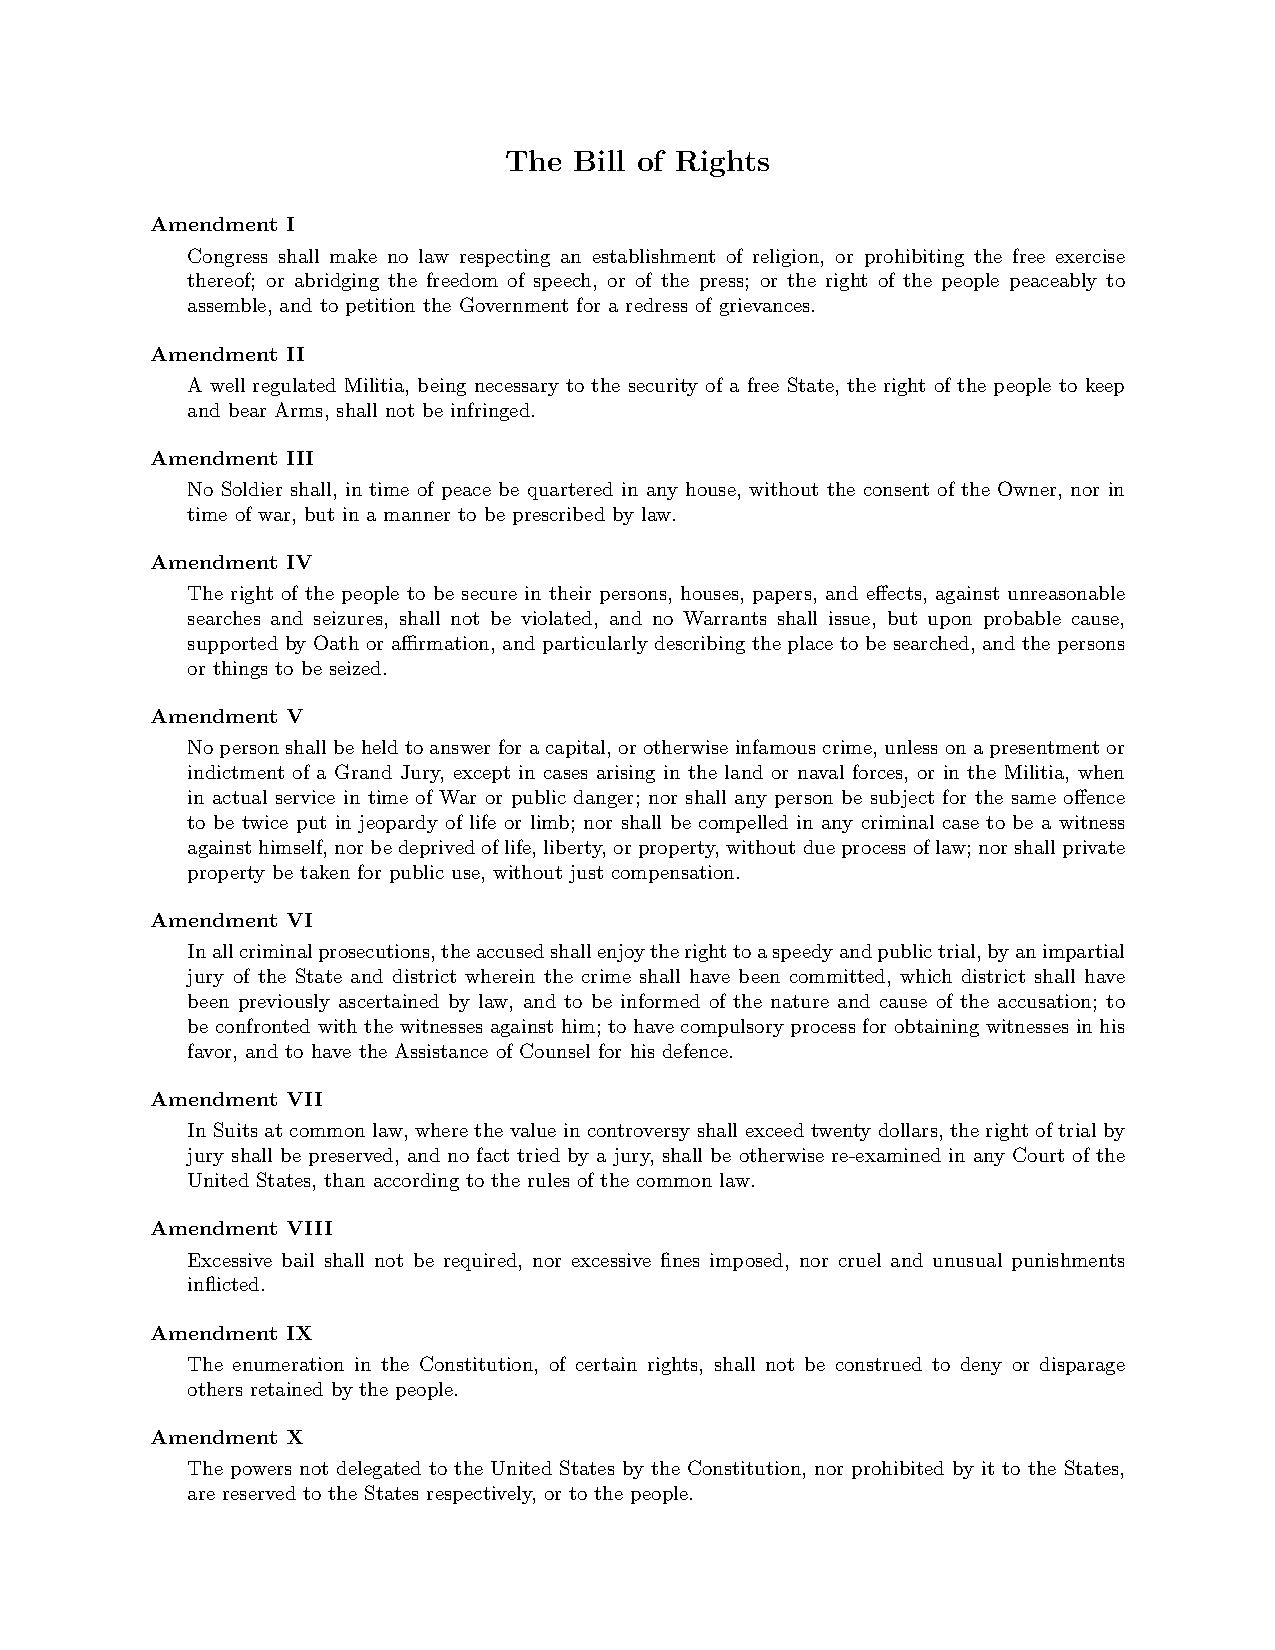
\includegraphics[trim=.9in .9in .9in .9in,clip,
        height=7.8in]{figs/rights}}
\caption{The Bill of Rights}
\label{fig:rights}
\end{figure}
\end{verbatim}

\begin{figure}\centering
\fbox{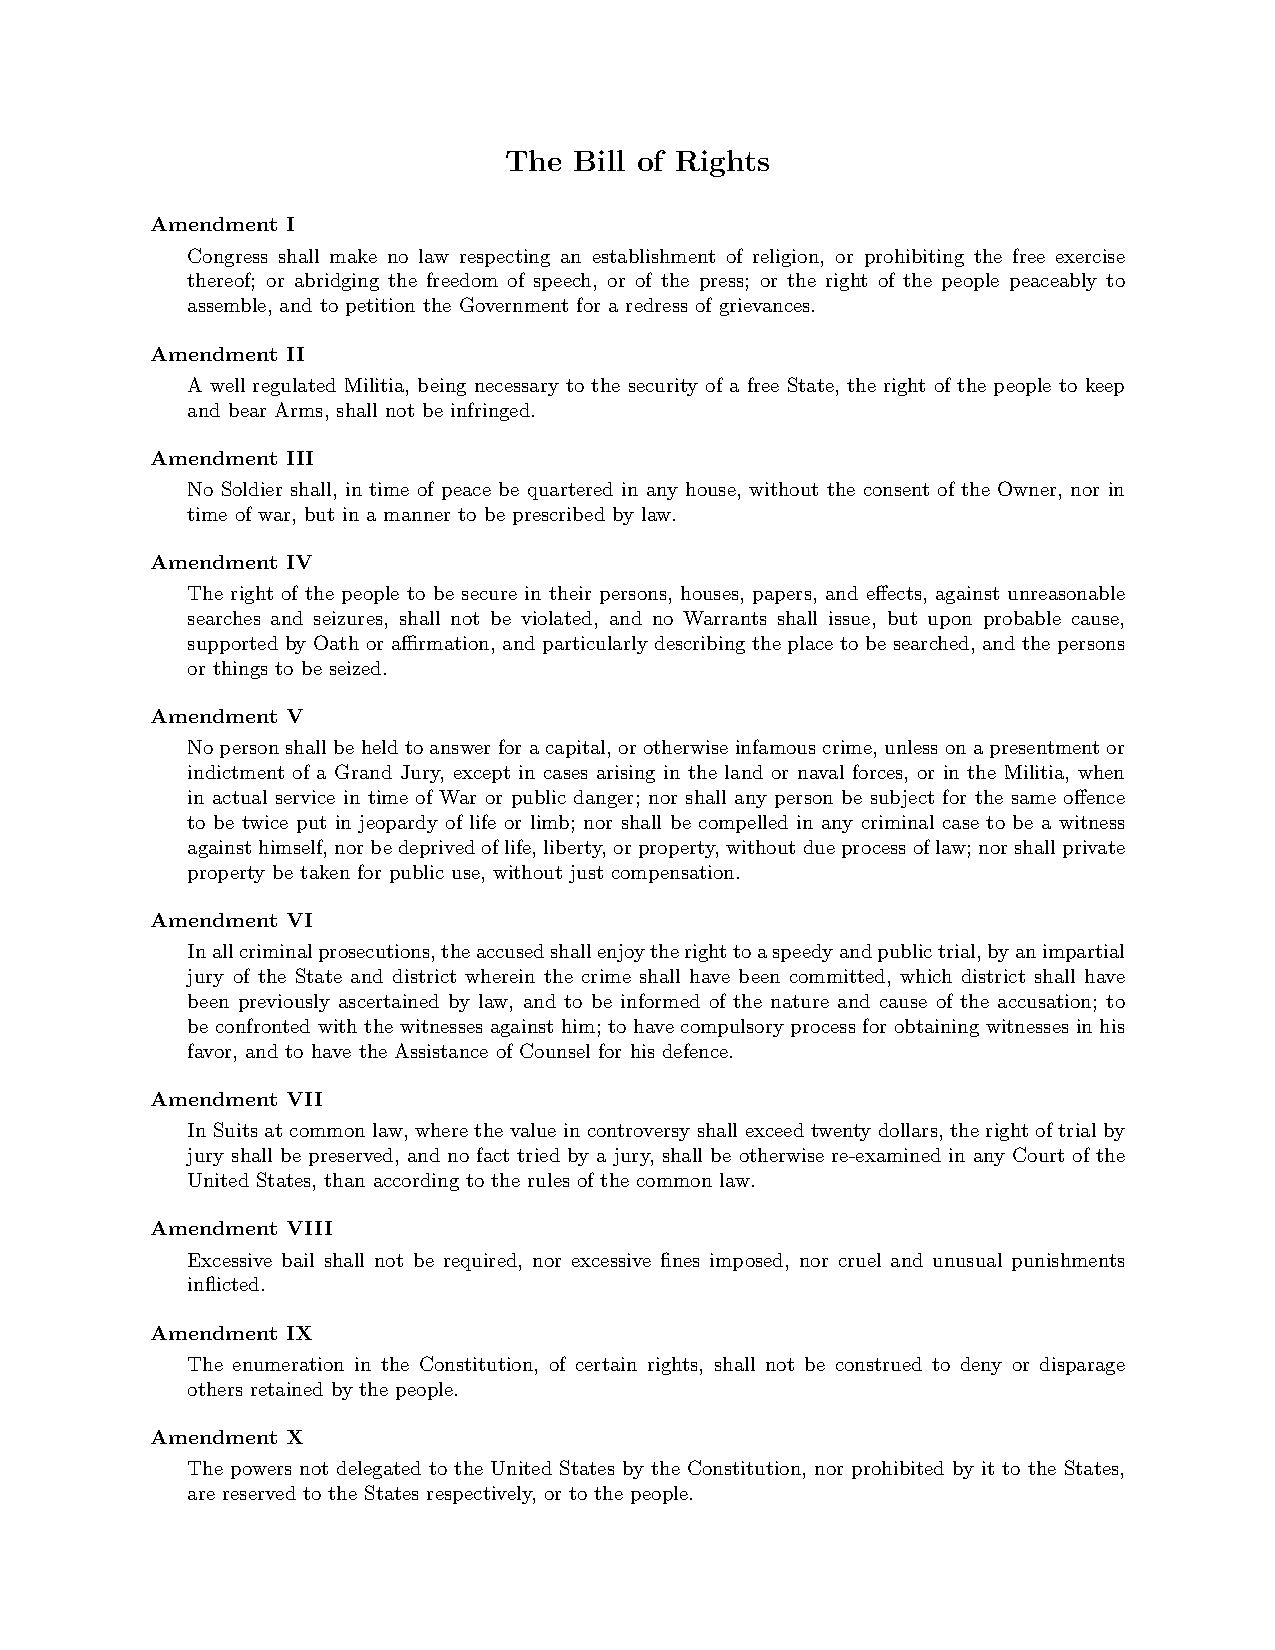
\includegraphics[trim=.9in .9in .9in .9in, clip,
           height=7.8in]{figs/rights}}
\caption{The Bill of Rights}
\label{fig:rights}
\end{figure}

\section{Musical Examples}
If your thesis or dissertation requires you to include musical
examples, the \pkg{fsuthesis} class has an environment already set up
for you.  Each musical example should be in its own PostScript
\acro{EPS} file or \acro{PDF} file (depending on the \pkg{graphicx}
driver you are using).  Then, rather than using the \lit{figure}
environment, you would use the \lit{musex} environment as demonstrated
here to create Example~\ref{mus:bass-ode}:
\begin{verbatim}
\begin{musex}
\begin{center}

\includegraphics{figs/freude}
\end{center}
\caption{The bass soloist's opening statement in the 9th Symphony.
  \label{mus:bass-ode}}
\end{musex}
\end{verbatim}

As with figures, the caption follows the graphic.  However, the
caption will be automatically titled with ``Example'' rather than
``Figure''.  If your document contains more than one musical example,
they can be listed in their own table by using the command
\verb|\listofmusex| in the front matter section of your document.

\begin{musex}
\begin{center}

\includegraphics{figs/freude}
\end{center}
\caption{The bass soloist's opening statement in the 9th Symphony.
\label{mus:bass-ode}}
\end{musex}

\section{Further Information}
This chapter intended to provide a brief overview of figure inclusion,
along with a few simple examples.  If your figure-insertion needs have
not yet been addressed, you should look up the document \textit{Using
  Imported Graphics in \LaTeX{} and pdf\LaTeX} by Keith Reckdahl,
which is part of the Comprehensive \TeX{} Archive Network (CTAN).
This document provides a wealth of detail about figure manipulation,
insertion, and placement.

In addition to the inclusion of external figures, \LaTeX{} provides
several environments and packages for creating figures mathematically
(usually technical line-drawings) within a \LaTeX{} document itself.
Investigate the \pkg{picture} package and its extensions \pkg{epic}
and \pkg{eepic}.  Other figures and text manipulations can be carried
out with the \pkg{pstricks} package.  The program \MP\ can generate
precise renderings of mathematical objects and diagrams.  And there
are many more utilities and packages to assist you.


